\documentclass[12pt]{article}

%==============Packages & Commands==============
\usepackage{graphicx}
\usepackage{fancyvrb}
\usepackage{tikz}
%%%<
\usepackage{verbatim}
%\usepackage[active,tightpage]{preview}
%\PreviewEnvironment{tikzpicture}
%\setlength\PreviewBorder{5pt}%

\usepackage{geometry}                		% See geometry.pdf to learn the layout options. There are lots.
\geometry{letterpaper}                   		% ... or a4paper or a5paper or ...
%\geometry{landscape}                		% Activat\usetikzlibrary{arrows}e for for rotated page geometry
%\usepackage[parfill]{parskip}    		% Activate to begin paragraphs with an empty line rather than an indent
\usepackage{graphicx}				% Use pdf, png, jpg, or eps§ with pdflatex; use eps in DVI mode
								% TeX will automatically convert eps --> pdf in pdflatex
\usepackage{amssymb}

\usepackage[ruled,vlined]{algorithm2e}
\usetikzlibrary{arrows}
\usepackage{alltt}
\usepackage[T1]{fontenc}
\usepackage[utf8]{inputenc}
\usepackage{indentfirst}
%\usepackage[longnamesfirst]{natbib} % For references
%\bibpunct{(}{)}{;}{a}{}{,} % Reference punctuation
\usepackage{changepage}
\usepackage{setspace}
\usepackage{booktabs} % For tables
\usepackage{rotating} % For sideways tables/figures
\usepackage{amsmath}
\usepackage{multirow}
\usepackage{color}
\usepackage{harvard}
\renewcommand{\harvardurl}{URL: \url}
\usepackage{dcolumn}
\usepackage{comment}
%\usepackage{fullwidth}
\newcolumntype{d}[1]{D{.}{\cdot}{#1}}
\newcolumntype{.}{D{.}{.}{-1}}
\newcolumntype{3}{D{.}{.}{3}}
\newcolumntype{4}{D{.}{.}{4}}
\newcolumntype{5}{D{.}{.}{5}}
\usepackage{float}
\usepackage[hyphens]{url}
%\usepackage[margin = 1.25in]{geometry}
%\usepackage[nolists,figuresfirst]{endfloat} % Figures and tables at the end
\usepackage{subfig}
\captionsetup[subfloat]{position = top, font = normalsize} % For sub-figure captions
\usepackage{fancyhdr}
%\makeatletter
%\def\url@leostyle{%
%  \@ifundefined{selectfont}{\def\UrlFont{\sf}}{\def\UrlFont{\small\ttfamily}}}
%\makeatother
%% Now actually use the newly defined style.
\urlstyle{same}
\usepackage{times}
\usepackage{mathptmx}
%\usepackage[colorlinks = true,
%						bookmarksopen = true,
%						pagebackref = true,
%						linkcolor = black,
%						citecolor = black,
% 					urlcolor = black]{hyperref}
%\usepackage[all]{hypcap}
%\urlstyle{same}
\newcommand{\fnote}[1]{\footnote{\normalsize{#1}}} % 12 pt, double spaced footnotes
\def\citeapos#1{\citeauthor{#1}'s (\citeyear{#1})}
\def\citeaposs#1{\citeauthor{#1}' (\citeyear{#1})}
\newcommand{\bm}[1]{\boldsymbol{#1}} %makes bold math symbols easier
\newcommand{\R}{\textsf{R}\space} %R in textsf font
\newcommand{\netinf}{\texttt{NetInf}\space} %R in textsf font
\newcommand{\iid}{i.i.d} %shorthand for iid
\newcommand{\cites}{{\bf \textcolor{red}{CITES}}} %shorthand for iid
%\usepackage[compact]{titlesec}
%\titlespacing{\section}{0pt}{*0}{*0}
%\titlespacing{\subsection}{0pt}{*0}{*0}
%\titlespacing{\subsubsection}{0pt}{*0}{*0}
%\setlength{\parskip}{0pt}
%\setlength{\parsep}{0pt}
%\setlength{\bibsep}{2pt}
%\renewcommand{\headrulewidth}{0pt}

%\renewcommand{\figureplace}{ % This places [Insert Table X here] and [Insert Figure Y here] in the text
%\begin{center}
%[Insert \figurename~\thepostfig\ here]
%\end{center}}
%\renewcommand{\tableplace}{%
%\begin{center}
%[Insert \tablename~\theposttbl\ here]
%\end{center}}

\newcommand\independent{\protect\mathpalette{\protect\independenT}{\perp}}
\def\independenT#1#2{\mathrel{\rlap{$#1#2$}\mkern2mu{#1#2}}}
\newcommand{\N}{\mathcal{N}}
\newcommand{\Y}{\bm{\mathcal{Y}}}
\newcommand{\bZ}{\bm{Z}}

\usepackage[colorlinks = TRUE, urlcolor = black, linkcolor = black, citecolor = black, pdfstartview = FitV]{hyperref}


%============Article Title, Authors==================
\title{\vspace{-2cm} Automated Citation Indexing of Government Documents} 


\author{ Ben Fisher \and Bruce Desmarais} \date{\today}



%===================Startup=======================
\begin{document}
\maketitle

%=============Abstract & Keywords==================

\begin{abstract}

 \noindent  We extract citations from government documents. \\~\\

\end{abstract}

Intended Journals \begin{itemize}
\item {\em Journal of Informetrics}
\item {\em Scientometrics}
\item {\em PLoS ONE altmetrics collection}
\item {\em WWW Workshop on Big Scholarly Data}
\item {\em PNAS}
\end{itemize}

\thispagestyle{empty}
\newpage
\doublespacing


\section{Introduction}
% write this as if the main goal is to extract scientific cites, with other references as an extra benefit
Assessing the impact of scientific research in applied contexts is challenging, but necessary in evaluating the returns to society from investing in basic science. The measures used to assess the scientific importance of basic research are largely derived from citation in the bibliographies of scientific papers. One of the major challenges in assessing impact outside of the scientific community is that applied users of basic science rarely produce systematic and publicly available bibliographies. One exception is the recent focus on patents \cite{huang2014,liaw2014,huang2015,wong2015}. One area of real-world impact of science that is highly relevant to all members of society is the use of science in the creation of government policy \cite{nrc2012}. Indeed, the technical basis of government regulations has grown so salient in recent decades that regulations are regularly challenged in court on the basis of the science underpinning major provisions \cite{ellig2013,morrall2014}. As such, while developing policies, government officials regularly create publicly available and heavily vetted documents in which they present the research on which a regulation is based. If we can systematically extract and organize this information, we can directly assess the impact of scientific research on public policy.

% We need to do this automatically
Our goal is to assess the degree to which a publication in a peer-reviewed scientific journal has been directly used in benefit-cost analyses conducted by policymakers. These benefit-cost analyses, termed ``Regulatory Impact Analyses'' (RIAs) in the US federal government, directly inform the process of crafting government regulations. It is now standard procedure in dozens of national governments, and many sub-national governments such as the US states, for policymakers to conduct a benefit-cost analysis to inform the provisions in government regulations \cite{hahn2007}. By indexing these analyses for citations to the scientific literature, we construct a measure of the degree to which an individual paper or journal, has directly informed the process of crafting government regulations. We build upon a dataset introduced by \cite{desmarais2014} in which citations from 104 RIAs covering major regulations passed by the US federal government during the period 2008--2012. Though feasible for small collections of benefit-cost analyses, hand-indexing would be prohibitively expensive for larger corpora, which could easily number in the tens of thousands if they covered longer spans of time, other nations, or subnational governments. We use the dataset introduced by \cite{desmarais2014} to train and evaluate procedures for automating citation indexing for RIAs. We then apply automated indexing to an expanded corpus of RIAs from the US federal government, and use these citations to construct a regulatory policy impact factor.

\subsection{Tasks}

\begin{itemize}
\item Write ``outline of the paper'' paragraph (BD)


\end{itemize}

\section{Literature Review}
The development of citation indexing has primarily focused on indexing scholarly citations in the confines of large-scale projects like \citeasnoun{garfield1964}'s Science Citation Index, which eventually morphed present Web of Science or \citeasnoun{lawrenceetal1999}'s Citeseer database. The process by which proprietary services like Web of Science or Google Scholar actually extract citations is opaque. The Citeseer project employs a heuristic, rule-based approach to identify citation strings within text. For example, the ParsCit parser developed by \citeasnoun{councilletal2008}, which Citeseer currently uses, identifies the bibliography of a paper by searching for ``bibliography'' or synonyms like ``references''. If one of these is found past the first 40\% of the paper, then the parser extracts all of the text past that line through the end of the paper or the appearance of another section heading, such as ``appendix''. The citation strings are then separated using regular expressions. 

There has been limited publicly available work done on improving automated citation indexing beyond the Citeseer project. Papers on citation metadata extraction generally rely on citation datasets downloaded from Citeseer or manually compiled datasets, rather than developing new methods for parsing documents themselves \cite{anzaroot2013}. Additionally, the automated citation indexing methods used by Citeseer and similar databases is tailored for extracting scholarly citations, making the application of existing algorithms problematic for extracting heterogeneous citations from government reports.

Citation indexing can be seen as a special case of token tagging in text (i.e., part of speech (POS)) tagging. Consider a document in which every word (or token) has a tag from a given tag set (e.g., POS = \{noun, verb, adjective,...,\}). The word ``run'', for example, would likely be tagged as a verb, but could also be tagged as a noun (e.g., ``I am going on a run''). Citation indexing could be seen as a two-part token tagging task. First, within a document, we need to tag tokens regarding whether they are within a citation instance, with adjacent sets of tokens in a citation instance representing a single citation. Second, after extracting citations, tagging the tokens within the citation index as title, author, etc. For our purposes, we really only need a tagger that performs well at the first task, as the second task can be performed by hand or with the assistance of other citation indexes (e.g., Google Scholar). The Stanford POS tagger can be used to train a tagger using a custom tag set \cite{toutanova2003}. We could use a grep for scientific cite titles in our hand-coded data to tag tokens as starting a cite title, within a cite title, ending a cite title and not in a cite title. Other tags may be useful, but whatever the tag set, we could train the Stanford Tagger and test extraction rules for automatically indexing cites.  


\subsection{Tasks}

\begin{itemize}
\item Review "altmetrics" lit (BD)
\item  read huang2014 and Liaw2014 to develop notes about framing and presenting the contribution (BF)

\end{itemize}

\section{RIA Description}

\section{Research Design}
We use 105 RIAs whose citations have already been extracted by hand as a test sample. The structure of these RIAs is very heterogeneous. They vary in length from a few dozen pages to hundreds of pages. References may appear in a reference section, in footnotes, or be scattered throughout the text. The citations of interest include both scholarly citations and non-scholarly citations, such as existing federal regulations, court cases, and treaties. The source documents are in PDF format, which we convert to plain text for the purposes of analysis using Apache Software's PDFBox program.\\ 

To assess how our own approach compares to existing citation indexing programs, we run the ParsCit program on the manually coded sample of RIAs. ParsCit was originally developed for indexing scholarly citations from journal articles for the Citeseer project \cite{councilletal2008}. In addition to extracting citations, the program also extracts citation metadata, such as author, article title, and journal. We do not expect it to handle metadata extraction for non-scholarly citations. However, it may be able to extract text containing non-scholarly citations, which could then be manually coded. This would greatly speed up the current coding process, which requires research assistants to read the entire document for citations. If ParsCit performs well enough at extracting all citation types, then there is no need to develop new indexing software for this project.\\

We use four different string distance metrics to measure similarity between the titles of manually collected citations and those of the citations collected by ParsCit: Levenshtein, Jaccard, Sorensen, and partial string similarity. Levenshtein distance is measured by calculating the number of insertions, deletions, or substitutions needed to turn one string into another string \cite{levenshtein1966}. To calculate the Jaccard distance, the number of characters shared by two strings is divided by the total number of characters and subtracted from 1 \cite{jaccard1901}. The Sorensen distance measure is very similar to the Jaccard measure. Instead of looking at the number of shared characters, the Sorensen measure calculates the number of shared bigrams. This number is multiplied by 2 and then divided by the total number of bigrams in each string and subtracted from 1 \cite{sorensen1948}. Except for Levenshtein distance, all measures fall on a scale of 0 to 1, with 0 indicating an exact match and 1 indicating two completely different strings. The Levenshtein measure is normalized to the same scale for the purposes of comparison. The final measure, partial string similarity, uses substring matching and measures the percentage of characters in string $a$ that appear in string $b$.\\

To determine which distance measure works best as a classifier in this case, we first hand code whether the best match from the ParsCit-collected citations suggested by each distance measure for each hand coding whether the suggested match is actually a match. The best distance measure is that which provides the most correct matches. We then determine a cutoff point for the best distance measure that which best divides matches from non-matches and apply it to the whole sample.\\


We can think of our use of Levenshtein distance to label a match as a diagnostic test with X\% accuracy. Given the standard testing adjustments \cite{pewsner2004}, we can say that ParsCit identifies A-B\% of all citations in the data.


\subsection{Tasks}

\begin{enumerate}
\item Make sure data we are using on articles comes from WebofScience via DOI download. BF send comma-separated list of DOIs to BD. BD return DOI-based data frame to BF.
\item Normalize journal impact factors by volume of articles published (BF). Get data on journals from JCR. For each journal, try to download number of articles published and impact factor data for each year going back as far as you can.
\item Calculate five year impact factor (BF).  For time T, the number of cites to that journal between T and T+4 (verify this shouldn't be T+5).
\item Create journal ranking scatterplot in hand-coded and parsCit coded (BF).
\item Calculate average difference in rank between hand-coded and Parscit coded (BF).
\item Need to figure out if cite records from ParsCit can pull DOIs from the web (BF).
\item What is the rate of article recovery if we use CiteULike matched records rather than ParScit matched records (i.e., re-do Figure 4 throwing out parscit-discovered records that cannot be found on CiteULike)? (BF) 
\item Get big trove of RIAs (BD)
\end{enumerate}



\section{Results}
We treat the values for each distance measure as pseudoprobabilities, which we use to generate Receiver Operating Characteristic (ROC) curves. Figure~\ref{fig:roc} displays ROC curves for each distance measure. The best measure is the one that has the greatest area-under-the-curve (AUC). In this case, partial string similarity and Levenshtein distance perform roughly the same, while Jaccard and sorensen measures do worse. We use Levenshtein distance due to its superior performance and wide use. Using the Levenshtein measure, we determine the ideal cutoff point by choosing the point that maximizes the sum of sensitivity and specificity. In this case, the best threshold is .6. Potential matches with a score below .6 are considered matches, while those above are considered non-matches.

Roughly $41\%$ of the hand-coded citations are also present in the ParsCit-extracted citations. Table~\ref{tab:focalhand} displays the number of matched citations by the major citation types\footnote{not all citations fell into one of these categories}. The major advantage of ParsCit should be it's ability to pick up scholarly journal citations. However, it actually performs quite poorly, picking up less than half of the scholarly citations present in the hand-coded dataset. This may be due to the fact that ParsCit was designed under the assumption that each document contains a reference section, which is not always the case with RIAs. Table~\ref{tab:bibmatch} displays the number of matches and total citations for RIAs with bibliographies and RIAs without, while Table~\ref{tab:bibtypes} displays matches by citation types for RIAs with bibliographies only.

We also look at how these metrics change over time. The sample of RIAs we use here covers 2008 through 2012. Figure~\ref{fig:yearlyaccuracy} shows the average accuracy of ParsCit for all citation types by year when compared to the hand coded data. Figure~\ref{fig:scholarlytotals} and Figure~\ref{fig:scholarlyaccuracy} look at scholarly citations specifically. The former shows the total number of scholarly citations from the hand coded data by year, while the latter shows the percentage of these that were actually picked up by ParsCit for each year. ParsCit maintains a fairly consistent accuracy of around 50\%. One caveat is that this is all under the same presidential administration, and these metrics may change with a change in president and consequent policies.

Figure~\ref{fig:impacts} shows journal impact factor statistics for the full sample of scholarly citations and various subsets of the data. These subsets include citations found by ParsCit, citations not found by Parscit, citations from RIAs with bibliographies, and citations from RIAs without bibliographies. Overall, the average impact factor across the different samples is fairly similar, with the found by ParsCit and no bibliography samples slightly higher on average. Table~\ref{tab:allimpact} and Table~\ref{tab:pcimpact} show the top journals for the full sample of scholarly citations and the sample of those found by ParsCit respectively. The two are quite similar and, and with one exception, consist entirely of scientific and health journals. \\

\begin{figure}
\begin{center}
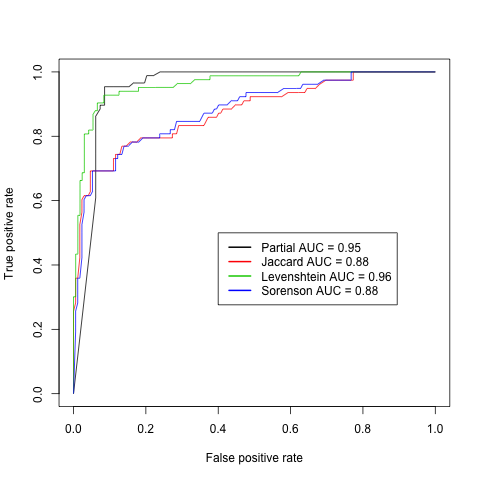
\includegraphics[height=8cm]{roc_curves.png}
\caption{ROC Curves}
\label{fig:roc}
\end{center}
\end{figure}

\begin{table}[ht]
\centering
\caption{Hand-coded citations matched by type}\label{tab:focalhand}
\begin{tabular}{lll}
  \hline
  \hline
 Type & Matched & Total\\
 \hline
Article & 96 & 188 \\
Book & 65 & 131\\
Court Case & 1 & 26\\
Database & 115 & 334\\
Government Report & 462 & 1308\\
Hearing & 16 & 45\\
Magazine/Newspaper & 10 & 13\\
NGO Report & 217 & 622 \\
Other & 183 & 640\\
Reference Manual & 14 & 67\\
Regulation & 46 & 296\\
RIA & 28 & 80\\
Scholarly Journal & 626 & 1209\\
  \hline
  \hline
\end{tabular}
\end{table}

\begin{table}[ht]
\centering
\caption{Hand-coded citations matched by presence of bibliography}\label{tab:bibmatch}
\begin{tabular}{lll}
  \hline
  \hline
 Bibliography? & Matched & Total\\
 \hline
 Yes & 1788 & 3340\\
 No & 227 & 1750\\
  \hline
  \hline
\end{tabular}
\end{table}

\begin{table}[ht]
\centering
\caption{Hand-coded citations matched for RIAs with bibliography}\label{tab:bibtypes}
\begin{tabular}{lll}
  \hline
  \hline
 Type & Matched & Total\\
 \hline
Article & 76 & 143 \\
Book & 45 & 80\\
Court Case & 0 & 2\\
Database & 92 & 208 \\
Government Report & 299 & 712 \\
Hearing & 13 & 20\\
Magazine/Newspaper & 5 & 5\\
NGO Report & 176 & 376 \\
Other & 166 & 398 \\
Reference Manual & 7 &  32\\
Regulation & 35 & 69 \\
RIA & 20 & 54\\
Scholarly Journal & 470 & 787\\
  \hline
  \hline
\end{tabular}
\end{table}

\begin{table}[ht]
\centering
\caption{Top Journals from Hand Coded Sample}\label{tab:allimpact}
\begin{tabular}{lll}
  \hline
  \hline
 Journal & Cites & Impact Factor\\
 \hline
Epidemiology & 62 & 6.196\\
Environmental Science and Technology & 56 & 5.330 \\
Environmental Health Perspectives & 35 & 7.977\\
American Journal of Respiratory and Critical Care Medicine & 33 & 12.996\\
Energy Policy & 30 & 2.575\\
Environmental Research & 30 & 4.373\\ 
American Economic Review & 3.673\\
Atmospheric Environment & 25 & 3.281\\
Health Affairs & 24 & 4.966\\
Journal of Environmental Economics and Management & 24 & 2.394\\
  \hline
  \hline
\end{tabular}
\end{table}

\begin{table}[ht]
\centering
\caption{Top Journals from ParsCit Sample}\label{tab:pcimpact}
\begin{tabular}{lll}
  \hline
  \hline
 Journal & Cites & Impact Factor\\
 \hline
Epidemiology & 30 & 6.196\\
Environmental Science and Technology & 27 & 5.330 \\
Environmental Health Perspectives & 25 & 7.977\\
Atmospheric Environment & 20 & 3.281\\
Journal of the American Medical Association & 19 & 35.289\\
Environmental Research & 30 & 4.373\\ 
American Journal of Respiratory and Critical Care Medicine & 33 & 12.996\\
New England Journal of Medicine & 14 & 55.873\\
Circulation & 12 & 15.073\\
American Journal of Public Health & 12 & 4.552\\
  \hline
  \hline
\end{tabular}
\end{table}

\begin{figure}
\begin{center}
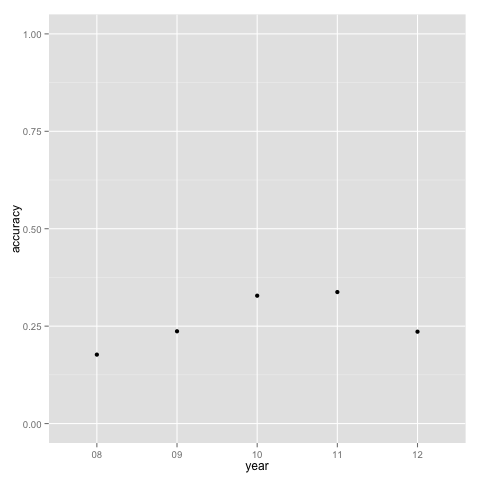
\includegraphics[height=8cm]{yearly_accuracy.png}
\caption{ParsCit Accuracy by Year}
\label{fig:yearlyaccuracy}
\end{center}
\end{figure}

\begin{figure}
\begin{center}
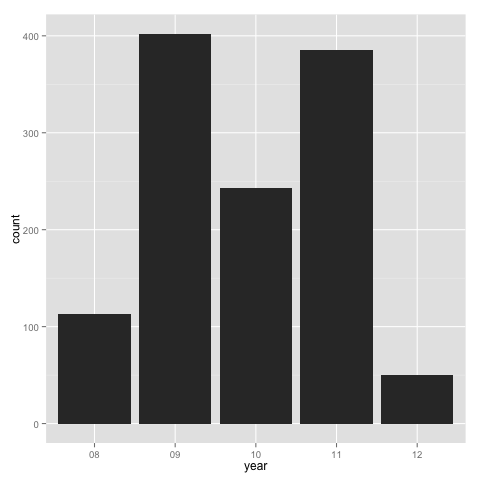
\includegraphics[height=8cm]{scholarly_totals.png}
\caption{Scholarly Citations by Year}
\label{fig:scholarlytotals}
\end{center}
\end{figure}

\begin{figure}
\begin{center}
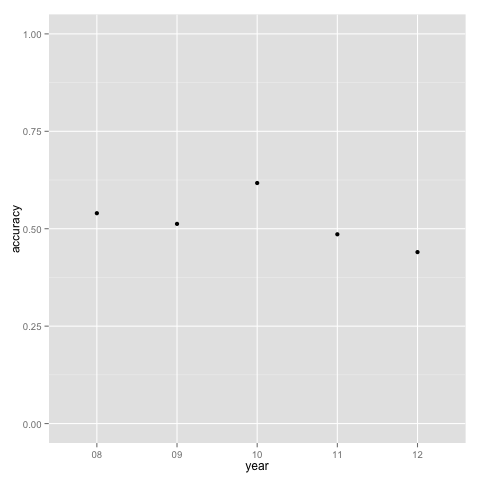
\includegraphics[height=8cm]{scholarly_accuracy.png}
\caption{ParsCit Scholarly Accuracy by Year}
\label{fig:scholarlyaccuracy}
\end{center}
\end{figure}

\begin{figure}
\begin{center}
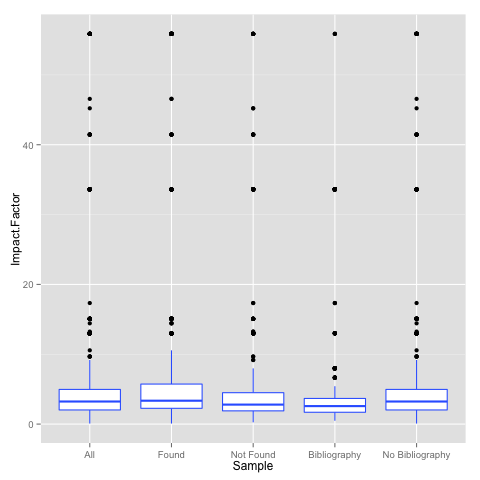
\includegraphics[height=8cm]{impacts.png}
\caption{Impact Factor by Sample}
\label{fig:impacts}
\end{center}
\end{figure}

\subsection{Tasks}

\begin{itemize}
\item Meet with Lee's student (Kyle?) to see how we can improve
\end{itemize}


\section{Conclusion}

\subsection{Tasks}

\begin{itemize}
\item Why the world needs this? (BD)
\end{itemize}


\clearpage
\singlespace
\bibliographystyle{apsr}
\nocite{*}
\bibliography{citationextraction}
\clearpage

\end{document}

